
% WARNINGS: 
%	    1. You must make sure that PDF output generated from this
%	       template is complete both when displayed with a viewer 
%	       (acroread, for example) and when printed on paper.
%	       LaTeX installations vary greatly and therefore it might 
%	       not be possible to get all proposals to come out 
%	       correctly with a single text page layout. 
%	       In some cases you will have to adjust the 
%	       \topmargin=-7mm command in the template to center the 
%	       text vertically in the page.  


\documentclass[12pt,a4paper]{article} 
\usepackage{times}
\usepackage{graphics,graphicx}
\usepackage[update,prepend]{epstopdf}
\usepackage[innercaption]{sidecap}
\usepackage{subcaption}
\usepackage{amssymb, amsmath}	       
\usepackage{xspace}				
\usepackage{natbibspacing, natbib}
\usepackage{aas_macros}
\usepackage{wrapfig}
\usepackage{floatrow}

\newcommand{\ncrit}{\mbox{$n_{\rm crit}$}\xspace}
\newcommand{\comol}{$^{12}$CO\xspace}
\newcommand{\Lsun}{\mbox{L$_{\odot}$}\xspace}
\newcommand{\LIR}{\mbox{$L_{\rm IR}$}\xspace}
\newcommand{\LFIR}{\mbox{$L_{\rm FIR}$}\xspace}
\newcommand{\rarr}{$\rightarrow$}
\newcommand{\aco}{\mbox{CO($J$=1\rarr0)}\xspace}
\newcommand{\bco}{\mbox{CO($J$=2\rarr1)}\xspace}
\newcommand{\cco}{\mbox{CO($J$=3\rarr2)}\xspace}
\newcommand{\eco}{\mbox{CO($J$=5\rarr4)}\xspace}
\newcommand{\rot}[3][HCN]{\mbox{#1($J$=#2\rarr#3)}\xspace} 
% default HCN; usage \rot[HCN]{3}{2} or \rot[\hcop]{4}{3}
\newcommand{\ahcn}{HCN($J$=1\rarr0)\xspace}
\newcommand{\dhcn}{HCN($J$=4\rarr3)\xspace}
\newcommand{\hcop}{HCO$^+$\xspace}
\newcommand{\ahcop}{\mbox{HCO$^+$($J$=1\rarr0)}}
\newcommand{\dhcop}{HCO$^+$($J$=4\rarr3)\xspace}
\newcommand{\Lp}[1][CO]{\mbox{$L^{\prime}_\textrm{\fontsize{8pt}{12pt}\selectfont{#1}}$}}
\newcommand{\LpU}{\mbox{K\,\,km\,\,s$^{-1}$\,\,pc$^2$}}
\newcommand{\kms}{km\,s$^{-1}$\xspace}
\newcommand{\pmOne}{\mbox{$^{-1}$}\xspace}
\newcommand{\Fig}[1]{Fig.~\ref{fig:#1}}
\newcommand{\Eq}[1]{Equation~\ref{eq:#1}}

%Compact BIB%%%%%%%%%%%%%%%%%%%%
\citestyle{aa}	
\bibliographystyle{apj_w_etal_3auth}

\usepackage{paralist}

\renewenvironment{thebibliography}[1]{%
%\section*{\refname}%
%  {\normalsize {\textbf{References:}}}
  \let\par\relax\let\newblock\relax%
  \inparaitem[{[}1{]}]}{\endinparaitem}
%%%%%%%%%%%%%%%%%%%%%%%%%%%%%


%%%%%%%%%%%%%%%%%%%%%%%%%%%%
%%%%%% Page dimensions %%%%%
%%%%%%	DO NOT CHANGE  %%%%%
%%%%%%%%%%%%%%%%%%%%%%%%%%%%

\textheight=247mm
\textwidth=180mm
\topmargin=-7mm
\oddsidemargin=-10mm
\evensidemargin=-10mm
\parindent 10pt

\renewcommand\floatpagefraction{.9}
\renewcommand\topfraction{.9}
\renewcommand\bottomfraction{.9}
\renewcommand\textfraction{.1}
% between fig
\setlength{\textfloatsep}{10pt plus 1.0pt minus2.0pt}
\setlength{\floatsep}{10pt plus 1.0pt minus 2.0pt}
\setlength{\intextsep}{10pt plus 1.0pt minus 2.0pt}
\setlength{\parskip}{0.01em}
\usepackage[small,tiny,compact]{titlesec}

\begin{document}
\pagestyle{plain}
\pagenumbering{arabic}
 
\begin{center}
{\large{\bf
{ 
Molecular gas dynamics and AGN/starburst mechanism in a
strongly-lensed wet merger: bridging the gap between local ULIRGs and high-z systems}
}}
\end{center}
\vspace{-0.545em}
\centerline{\normalsize{\bf PI: 
{T. K. Daisy Leung}}} 
%%%%%%%%%%%%%%%%%%%%%%%%%%%%%%%%%%
\vspace{0.1em} {\bf Missing link between mergers/ULIRGs and their high-z analogues} 
Ultraluminous infrared galaxies (ULIRGs: \LIR$\geq$10$^{12}$\Lsun) have been
regarded as analogues of high-redshift (z) starbursts given the
similarities in their interstellar medium (ISM; e.g. \LIR/\Lp).
As such, detailed studies 
of ULIRGs are important 
to gain more detailed insight into the early universe and in studies of galaxy evolution over cosmic time.
Since mergers are believed to play an important role in giving rise to these dusty galaxies
(e.g. Sanders \& Mirabel 1996). Yet, merger-induced effects on the physical mechanisms and chemistry 
that drive the 
%intense 
starburst (SB) and active galactic nucleus (AGN) activities on small scales are still unclear.
Thus characterizing the properties of the molecular gas that fuels star-formation (SF) and AGN is
crucial to understand the interplay between AGN and SB
and their relation to the ISM properties of galaxies across cosmic time.

While the ISM in local ULIRGs has been studied in great detail,
forming a rich inventory of molecular transitions that serves as the template for 
studying high-z galaxies 
\citep[e.g.][]{Rangwala15a}, a wide knowledge gap persists
between $z$=0 and the epoch when most stars are formed in the universe ($z$$\sim$2). 
Hence, understanding galaxy populations at which
the build-up of stellar mass 
is steeply rising is critical and we here aim to bridge this gap by testifying
correlations and properties found locally out to high redshift by observing the 
dynamical structure and properties of the ISM of
the quadruply lensed galaxy RXJ1131-1231 and its dust-obscured 
companion at $z_{\rm CO}$$\sim$0.65.

\noindent {\bf Molecular gas in AGN/SB} 
Owing to the high molecular gas fractions in ULIRGs,
% and their high-z analogues, 
their extreme SFRs are a natural consequence of either gas is being converted into stars
more efficiently and/or their molecular gas content. Fragmentation
of giant star-forming clumps and turbulent conditions are also expected 
from gravitational instability of these gas-rich bodies. 
In fact, studies of the ISM kinematics at $z$=1-2 find clumps of size scale
 $\sim$few kpc \citep{Swinbank12a, Swinbank12b}. 
Resolving the gas dynamics on hundred pc scales is therefore an important first step
to understanding the mechanisms and physical processes taking
place on different scales and how the ISM physical conditions 
are related to the SB in ULIRGs at this epoch. %(when the SFR density is steeply rising).

While \comol emission traces the total molecular distribution and dynamics,
high-dipole moment molecules such as HCN and \hcop are expected to trace the 
%properties of the 
denser, actively star-forming gas. Indeed, a tight correlation between \ahcn and \LIR 
(proxy for SFR) has been found in nearby galaxies and local giant molecular 
clouds (GMC; \citealt[hereafter GS04]{Gao04a}; \citealt{Wu05}), 
suggesting HCN is a faithful tracer of the star-forming dense gas.
% and that the origin can be attributed to the fundamental units of star formation. 
However, \dhcn observations of (U)LIRGs have revealed a wide range of
excitation conditions 
%for their dense gas phase 
that may render the ground state transition of 
HCN and \hcop poor proxies of the dense gas mass \citep[hereafter P07]{Papadopoulos07a}.
In this light, higher-$J$ transitions (e.g. $J$=4\rarr3) 
% are necessary to scrutinize the reliability of using the ground state 
have been suggested to be better probes
% dense gas mass tracers since the mid-$J$ transitions
since they trace the much denser gas (n$\gtrsim$10$^5-$10$^7$ cm$^{-3}$) that is 
thought to be the immediate fuel for SF in turbulent GMCs \citep{Shirley03a, KM05}. 
This has been supported by the linear correlations found in 
\LIR-\Lp[\dhcn] and \LIR-\Lp[\dhcop] \citep[hereafter Z14]{Zhang14a}.
Since the 
ground state lines are redshifted to frequencies beyond the spectral coverage of ALMA
at $z$$>$0.06, it is also necessary to establish diagnostics using these mid-$J$ lines to 
study distant galaxies.
Additionally, due to the difference in abundances and excitation conditions of HCN and \hcop
in star-forming versus AGN regions, the line 
% ratios \ahcn/HCO$^+$($J$=1\rarr0) \citep{Kohno05a, Imanishi10, Izumi13a} and
ratio \dhcn/\dhcop \citep{Imanishi14a, GB14a, Viti14a} have been 
proposed as
%  diagnostic tools 
a diagnostic tool to reveal deeply buried AGNs at the cores of ULIRGs \citep{Izumi16a, Imanishi16a}.
% separate emission originating from AGN and SB
% Recent studies have
% extended this diagnostic to using the J=4\rarr3 transitions 
%\citep{Imanishi14a, GB14a, Viti14a}, 
% where an elevated line ratio is seen in AGNs, suggesting
% it can be used to reveal deeply buried AGNs at the cores of ULIRGs \citep{Izumi16a, Imanishi16a}.

Prior to ALMA, studies of dense gas were largely limited to the local universe ($z$$\lesssim$0.1) 
with only five detections
%IR-luminous lensed galaxies detected 
at $z$$\gtrsim0.3$ 
(\citealt{Riechers06a, Riechers07a, Riechers10a, Wagg05a, Gao07a}).
Moreover, none of these 
%high-z detections 
spatially resolve the emission, rendering it difficult 
to draw conclusions on the dense gas properties of galaxies at high redshift. 
Even with ALMA, such studies will remain challenging, but by combining with
the magnification provided by gravitational lensing and the exceptional spatial resolution and sensitivity of ALMA, 
studies
of dense molecular gas in distant galaxies are now possible, as proposed here.

%%%%%%%%%%%%%%%%%%%%%%%%%%%%%%%%%% 
% \section*{Science Target RXJ 1131-1231: a demonstrative case at high-z}
% \vspace{-0.25em}
\noindent {\bf Science Target RXJ 1131-1231: a demonstrative case at high-z}
\vspace{-0.6em}
%\begin{figure}[!tbhp]
%\centering
%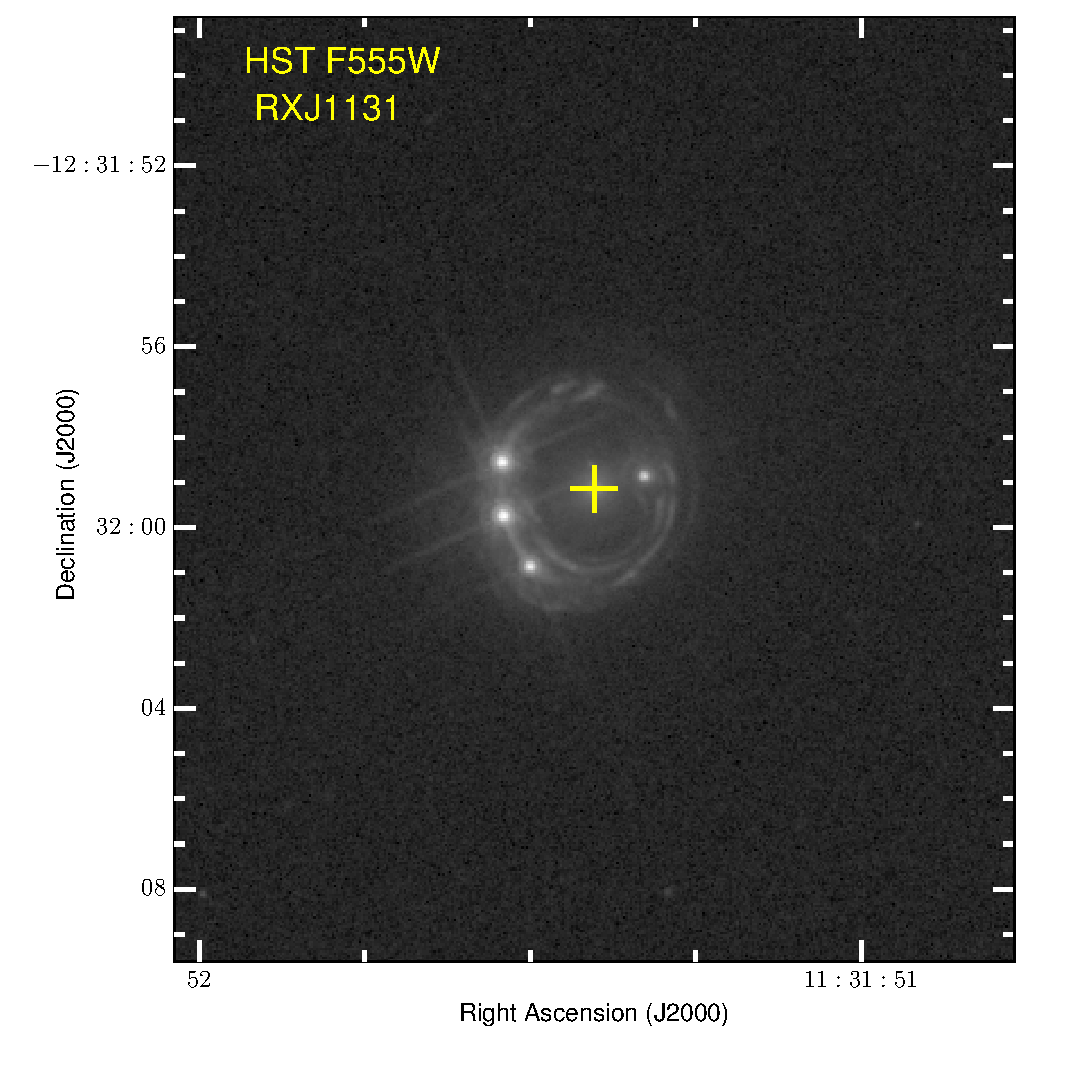
\includegraphics[trim= 10 20 15 0, clip, scale=0.3]{Fig/F555W} % &
%\hspace{-0.5em}
%\includegraphics[trim= 10 0 0 0, clip, scale=0.37]{Fig/Manipulate_figsCROP}
%\vspace{-1em}
%\caption{ \fontsize{10pt}{12pt}\selectfont 
%{
%\textbf{Stellar light distribution in the AGN host galaxy of RXJ 1131-1231 and its reconstructed source plane
%morphology}
%{\em Left:} The rest-frame UV emission (tracing recent star formation) 
%is lensed into an almost complete Einstein ring with diameter $\sim$ 3.8". 
%{\em Right:} Lens modeling of the optical emission identifies complex structure in the host galaxy and
%an optically faint companion (white; \citealt{Claeskens06a}), 
%which we have recently confirmed by modeling \bco emission detected with NOEMA
%(\Fig{combine}; Leung \& Riechers, in prep.). 
%We here propose to study
%the ISM conditions in this AGN-starburst composite system and offers an unparalleled
%view into the early universe, with finer
%detail than otherwise possible with current facilities. 
%}
%\label{fig:HST}}
%\end{figure}

\begin{figure}[!tbhp]
\centering
\hspace{-0.85em}
\floatbox[{\capbeside\thisfloatsetup{capbesideposition={right,center},capbesidewidth=0.445\textwidth}}]{figure}[\FBwidth]
{
\vspace*{-0.55em}
\hspace{-0.435em}
\raggedleft
\caption{ \fontsize{10pt}{12pt}\selectfont 
{
\textbf{Stellar light distribution in the AGN host galaxy of RXJ 1131-1231 and its reconstructed source plane
morphology}
{\em Left:} The rest-frame UV emission (tracing recent star formation) 
is lensed into an almost complete Einstein ring with diameter $\sim$3.8". 
{\em Right:} Lens modeling of the optical emission identifies complex structures in the host galaxy and
an optically faint companion (white; \citealt{Claeskens06a}), 
which we have recently confirmed by modeling \bco emission detected with NOEMA
(\Fig{combine}; Leung \& Riechers, in prep.). 
We here propose to study
the ISM conditions in this AGN-starburst merger and offers an unparalleled
view into the early universe, with finer
detail than otherwise possible with current facilities. 
}
\label{fig:HST}}}
{\hspace{-1em}
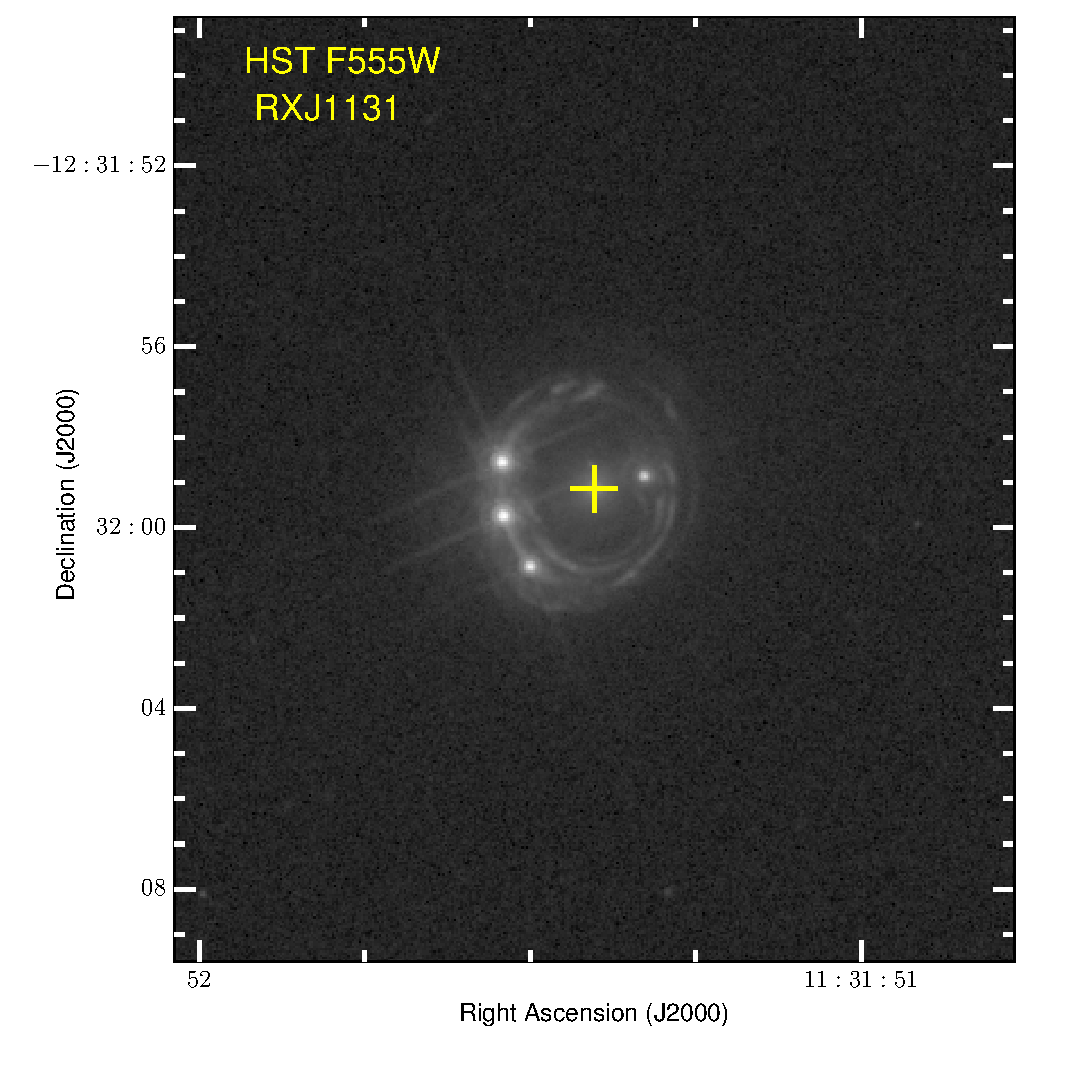
\includegraphics[trim= 10 20 15 0, clip, scale=0.28]{Fig/F555W}
\hspace{-1.5em}
\includegraphics[trim= 10 0 0 0, clip, scale=0.3]{Fig/Manipulate_figsCROP}
\vspace{-1.0em}
\hspace{-0.5em}
}
\end{figure}
\vspace{-0.8em}
RXJ 1131-1231 is a quadruply imaged AGN with its host galaxy lensed 
into a partial Einstein ring (\Fig{HST}). 
HST observations (rest-frame UV) have revealed distinct emission 
from recent star formation (lensing arcs) and from the AGN (bright knots) in the background galaxy \citep{Sluse03a},
demonstrating the great potential for probing its
ISM conditions in detail. Lens modeling carried out on optical images shows
that the AGN resides in a star-forming region of size $\sim$1 kpc
% $\sim$0.15" (without lensing magnification)
in its host galaxy, which itself is 7 kpc across, % $\sim$ 1 " (without lensing)
and made it possible to identify
seven distinct structures in the source plane (\Fig{HST}). Remarkably, emission 
%originating 
from 
a spatially offset region ($\sim$2.4 kpc away from the AGN host galaxy) has been identified and found 
to be $\sim$700 pc in size \citep{Brewer08a}, indicating a 
%nearby 
companion galaxy. 
We have recently confirmed that both galaxies are at the same redshift by detecting their 
\rot[CO]{2}{1} emission and lens-modeling their gas distribution 
in velocity space (\Fig{combine}f), and verfiied
that the both are gas-rich (Leung \& Riechers, in prep.). 
Our SED modeling of the dust continuum emission up to 500\,$\mu$m finds $L_{\rm IR}\sim6\times$10$^{12}$\Lsun 
(corrected for lensing). Hence, this target is a gas-rich ULIRG merger at $z$$\sim$0.7 caught in the act. 

%%%%%%%%%%%%%%%%%%%%%%%%%%%%%%%%%%
% \section*{Proposed Observations and Immediate Objectives}
% \vspace{-0.25em}
\noindent {\bf Proposed Observations and Science Goals}
We here propose to map (1): \eco at 0.15" resolution ($\sim$500pc at $z$$\sim$0.7 in the source plane) and 
(2): \dhcn and \dhcop emission and the underlying continuum at 0.7" resolution (2.5 kpc in the source plane).
The continuum traces the dust emission, 
providing better constraints on the the gas-to-dust ratio, dust temperature(s), dust mass,
and its spatial extent (and thus the surface density of the SFR).
%($\Sigma_{\rm SFR}$).
These quantities are key to investigate how the ISM % conditions 
vary as galaxies evolve across cosmic time.
In conjunction with the large set of ancillary data from
rest-frame UV to radio wavelength and our recent observations of \bco and \rot[CO]{3}{2}, our
proposed observations are designed to investigate 
% carry a detailed investigation of 
the gas-rich merger aspects listed as follows.

\underline{\bf Dynamics and kinematics:}
Our recently obtained \bco data shows an asymmetric double-horned line profile (\Fig{combine}a). Given
the 1$^{\rm st}$ moment map observed and the velocity gradient
across the source plane in our model (\Fig{combine}c \& \ref{fig:combine}f), this is indicative of
a kinematically ordered %(reminiscent of a rotating disk) 
galaxy but its emission has been lensed differentially. 
Limited by the spatial resolution of this data, it is insufficient to infer the true 
kinematics due to beam smearing.
Furthermore, the unusually high velocity dispersion 
$\gtrsim$400\kms at the central region (\Fig{combine}d) hints at 
perturbations from the AGN and/or
internal turbulence
% motion 
due to interactions with the companion
and/or instability due to the huge gas reservoir.
Thus higher-resolution imaging, as proposed here, is needed
% will allow us to
to distinguish 
%the major mechanism driving the starburst: 
between a merger-driven and a turbulent clumpy disk starburst, 
since we will be able to obtain a detailed
dynamical lens modeling of the system, probing at sub-kpc scale. % probe down to 0.15" <-> 500 pc

The \eco observations will be tracing emission on the size scale of high-z GMCs, 
% complementary to the optical images,
allowing us to compare the spatial distributions between recent star-formation (from HST) and star-forming 
gas clumps. Since \eco, HCN and \hcop trace the warm, excited, dense molecular gas,
this will as well allow us to compare against the relatively unperturbed large-scale 
molecular environment and dynamical mass using our existing 
low-$J$ CO data.
Such comparisons are the key to understand different processes %and timescales 
regulating star-formation 
in ULIRGs/mergers and examine how they differ from other galaxy populations.

\underline{\bf AGN/SB diagnostic:}
At the proposed resolution, we will be able to distinguish \dhcn and \dhcop
emission originating from the AGN host galaxy (and within) and from its companion.
%  as well as 
% resolving emission within the AGN host galaxy.  
By observing spatial variations in this line ratio across the AGN host galaxy, 
we will be able to assess its fidelity as an AGN/SB diagnostic,
at higher redshift than current studies, since
an elevated \dhcn/\dhcop is expected in nuclear regions near an AGN. 
By measuring this ratio in the companion, we will as well 
examine the possibility of a heavily-obscured AGN at its center.
Since the HCN vibrational line (v$_2$=1) falls within the targeted frequency range, 
we will use it to independently confirm the AGN in the companion, given that this line is excited by infrared 
pumping (easily achieved near an AGN) and is the cause of the elevated \dhcn/\dhcop% , as observed in AGNs 
\citep{Sakamoto10a,Imanishi13a}.
% The HCN vibrational line requires high temperature to excite and has been detected in AGN host galaxies, which
% has been attributed to arise/excited by IR radiative pumping near AGNs 
% excited by AGN-heated hot dust providing IR radiative pumping.

The high spin rate of the central black hole in RXJ1131-1231 (over half the speed of light; \citealt{Reis14a})
suggests that the black hole has grown via merger (i.e., the 
% background 
galaxies may have already encountered previously).
In this scenario, we might be witnessing a
second encounter of two AGN host galaxies if 
we find evidence of a buried AGN in the companion, 
which the proposed observations are needed to provide such clues.
%%%%%%%%%%%%%%%%%%%%%%%%%%%%%%%%%%%%%%

\underline{\bf Line ratios and physical conditions:}
[In addition, we will measure spatially resolve line ratios (HCN/CO and \hcop/CO) within the AGN host galaxy
as proxies of its very dense (cores; $\sim$10$^5$-10$^7$ cm$^{-3}$) versus the less dense (clumps; $\sim$10$^4$
cm$^{-3}$) gas content and their spatial distributions.]
OR 
[In addition, we will measure spatially resolve line ratios (HCN/CO and \hcop/CO) within the AGN host galaxy
to constrain the density gradients from $n$$\sim$10$^5$-10$^7$ 
%cm$^{-3}$
to $\sim$10$^4$cm$^{-3}$.]

% kinematics
We will also measure the linewidths of the very dense gas (traced by HCN and \hcop), 
the excited gas (traced by \eco), and the more-extended, less-perturbed 
molecular gas (traced by low-$J$ CO) at various locations to constrain 
the kinematics and relative mass-fractions of different gas phases, 
which are indications of the evolutionary stage of a galaxy.
% XDR versus PDRs
Since \eco is excited in higher temperature than the HCN and \hcop lines (e.g. in 
X-ray dominated regions (XDRs) near an AGN), 
variations in HCN/CO will allow us to constrain the spatial extents of photon dominated regions
 (PDRs from starbursts) and XDRs.
% (HCN/CO to be smaller for XDR than PDR because HCN is 
% boosted in high column density gas and CO more excited in high Tkin)
Due to differential lensing, we will be able obtain kinematical information
on spatial scales smaller than the beam, as seen in our 
\bco data (\Fig{combine}b \& \Fig{combine}c; the blue-shifted emission
arises from a region that is positioned differently with respect to the caustic
than the red-shifted emission), thereby
% and thus recover structural details and kinematics in finer detail than otherwise possible
enabling us to probe the aforementioned variations 
and gradients in the inner molecular disk (near the AGN). 

Differential lensing between HCN, \hcop, and CO emission is also expected 
as they trace different emitting regions and are arising from two galaxies. 
Hence, high spatial resolution is necessary to accurately measure their intrinsic 
line fluxes (free from differential
lensing biases) as it enables a detailed lens modeling on each line emission.
% surface brightness maps of HCN and \hcop
% By measuring the differences in their surface density ratios (
%  $\Sigma_{\rm HCN}$/$\Sigma_{\rm CO}$ and  $\Sigma_{\rm HCO^+}$/$\Sigma_{\rm CO}$),
Such measurements are vital to reveal how galaxy interactions drive gas into 
inner disks to initiate starbursts and AGN activities and how the ISM differ from 
normal star-forming galaxies.
% under the influence of an AGN and interactions with a companion. 
% with lower uncertainties because surface density is conserved in lensed, but flux is boosted.  
% CO SLED
We will also combine \eco with our existing CO data to constrain the gas density (n$_{H_{2}}$) 
and kinetic temperature by performing radiative transfer modeling. 

\underline{\bf The SK Law:}
The Schmidt-Kennicutt (SK) relation (%``Star-formation law"; 
$\Sigma_{\rm SFR}$=$A\Sigma^N_{\rm gas}$)
is one of the key ingredients
for theoretical models as it encodes the physical processes and timescales
regulating star-formation and their dependence on the ISM 
(e.g. \citealt{Narayanan14a}).
% lot of studies on
% how the power law index of KS law determined from observations should change depending on
% the critical density of the tracer used to probe the SF gas (e.g. Krumholz \& Thompson 07, Narayana+08)
% How SFR density should dependent on the global dynamical time scales in normal galaxies and in
% merges
However, the surface densities of gas at high densities (\ncrit$\sim$10$^7$cm$^{-3}$; 
$\Sigma_{\rm dense}$; and thus $\Sigma_{\rm SFR}\propto
\Sigma^N_{\rm dense}$) are currently poorly constrained due to the lack of 
(spatially resolved) observations of the much weaker emission 
from high critical density tracers. %(see right of \Fig{SF}).
It is thus unclear how the power-law index of the SK law should change depending on
the critical density of the tracer used to probe the SF gas \citep[e.g.][]{KT07a}.
and how the SFR surface density should depend on the global 
dynamical time scales in normal galaxies and in merges.
% To alleviate poorly-constrained SK law with the lack of observational data
% (on the SK relation), 
To further underline the problem, the integrated form 
(log\LIR=$\alpha$ log\Lp[X]+$\beta$; \citealt{SK})
% \LIR-\Lp[X]) 
has been commonly used as a proxy to the true SK relation,
for which correlations found for dense gas tracers
are incompatible with model predictions \citep[\Fig{SF}; Z14;][]{Greve14a}
and largely based on constraints % on the SK relation 
from local galaxies. 
% thus the linear correlations may not hold at earlier epochs. % (\Fig{SF}).
At the proposed resolutions, we will spatially resolve, for the first time,
the {\it true surface density version of the SK relation} using tracers with \ncrit$\gtrsim$10$^5$cm$^{-3}$
in a high-z merger: $\Sigma_{\rm SFR}$$\propto$$\Sigma^N_{\rm CO(5\rightarrow4)}$
%\eco 
in each of the interacting galaxies, and 
$\Sigma_{\rm SFR}$$\propto$$\Sigma_{\rm HCN(4\rightarrow4)}$ and 
$\Sigma_{\rm SFR}$$\propto$$\Sigma_{\rm HCO^+(4\rightarrow3)}$
% \dhcn and \dhcop 
within the AGN host galaxy and investigate potential variations in the power-law index.
% This will allow us to investigate the 
% variations in the true spatially resolved SK relation for high density 
% (and hence star-formation modes) 
% and provide constraints on the index $N$ at high critical densities
% at higher redshift than existing work.

\begin{figure*}[!tbph]
\vspace{-1.5em}
\centering
% \includegraphics[trim=5 0 435 0, clip, width=0.2\textwidth]{Fig/denseSK.eps}
\includegraphics[trim=15 0 5 10, clip, width=0.23\textwidth]{Fig/Zhang}
\hspace{-0.5em}
% \includegraphics[trim=20 5 5 10, clip, width=0.22\textwidth]{Fig/Zhang2}
\includegraphics[trim=117 5 5 10, clip, width=0.203\textwidth]{Fig/Zhang2}
\includegraphics[trim=10 0 0 5, clip, width=0.33\textwidth]{Fig/Greve14Fig2}
\includegraphics[trim=15 0 5 10, clip, width=0.22\textwidth]{Fig/SFRSD} % Garcia-Burillo+12
\caption{ \fontsize{10pt}{12pt}\selectfont {
{\em Left: } 
\textbf{The SK proxy: log \LIR = $\alpha$ log \Lp[X]+$\beta$.}}
Linear correlations in \LIR-\dhcn and \LIR-\dhcop have been established toward nearby galaxies 
(Z14), suggesting a single star-formation efficiency for all galaxies
and demonstrating the utility of mid-$J$ lines in tracing 
the star-forming dense gas, which will be routinely mapped in high-z galaxies with ALMA.
{\em Middle panels:} \textbf{Constraints on the SK relation 
with line transitions of different \ncrit.}
Most observations are incompatible with model predictions (gray shaded),
especially for \dhcn
\citep{Greve14a}. 
% Our proposed observations will provide constraints on
% the slope ($alpha$) at high critical density. 
{\em Right:} \textbf{The true SK relation for the dense gas using HCN($J$=1\rarr0)}
%: $\Sigma_{\rm SFR}$=$\Sigma^N_{\rm gas}$}
While constraints on the power-law index from gas of different densities are important for star-formation 
models,
current studies are only able to constrain the true SK law using the ground state HCN line 
(\ncrit$\sim$10$^{4}$) and largely limited to nearby measurements
%  due to the lack of spatially resolved observations of
% dense gas tracers at high redshift 
\citep{GC08a}. 
% It also appears that (U)LIRGs (\LIR$>$$10^{11}$\Lsun)
% and normal (\LIR$<$$10^{11}$\Lsun) galaxies have do not follow the same power law (different SFE).
Our proposed observations will, for the first time, spatially resolve the true 
SK relation with high critical density tracers in a merger at $z$$\sim$0.7, 
exploring potential deviations in SK relation at higher redshift, providing 
key constraints for models of galaxy evolution.
\label{fig:SF}}
\vspace{-0.85em}
\end{figure*}

%%%%%%%%%%%%%%%%%%%%%%%%%%%%%%%%%%%
\noindent {\bf Technical overview}
% We propose to observe the \eco line at 0.15" resolution
% and the \dhcn and \dhcop lines at 0.7", 
We estimate the line widths and fluxes 
% assuming a line width
% of 700\kms 
based on our \bco data, and a source size from our lens model.
%, which takes into account the asymmetric line emission and spatial extent due to differential lensing. 
We thus expect the source to be resolved over 153 beams 
and 7 beams at 0.15" and 0.7", respectively (see TJ for details). 
% We compute the target sensitivities for both science goals based on the \bco line flux. 
We adopt conservative 
line ratios measured for high-z galaxies for \eco line \citep[][]{CW13}
and those based on (U)LIRGs for \dhcn (GS04; P07).
For \dhcop, we adopt the line ratio \dhcn/\dhcop found in ULIRGs 
\citep{Greve09a}. 
We use the most stringent sensitivity estimates 
among \dhcn and \dhcop as our sensitivity goal for science goal $1$. %The latter sets the overall requirement. 
To secure enough S/N for lens modeling, 
we require a minimum of 8$\sigma$ of 0.47 mJy beam\pmOne and 0.07 mJy beam\pmOne
per 150 \kms channel 
%to reconstruct the dynamical structure in the source plane 
for the science goals, respectively. 
% We therefore request a \textbf{total time of 7.0 hours}.% to complete our science goals. 

%%%%%%%%%%%%%%%%%%%%%%%%%%%%%%
% closing
%\par 
%Our proposed observations present an exceptional opportunity to investigate
%the physical properties and dynamical structures of 
%%different gas phases in 
%the ISM in mergers at the cosmic epoch 
%where the SFR density is steeply rising \citep{LeFloch05a}, 
%connecting high redshift and nearby studies to improve our understanding of galaxy evolution.
%%Our proposed observations are vital
%%% between the \LIR, SFR$_{\rm IR}$, SFR$_{\rm UV}$, surface densities of SFR, CO, HCN and \hcop,
%%to provide constraints on the relation between the ISM and AGN/SB acitvities
%%on sub-kpc scales and on the mechanisms driving the vast SFR at earlier epochs, 
%%giving rise to the observed stellar-assembly history.
%%
%This will also % lay the groundwork to 
%% serve as a benchmark demonstrating
%demonstrate the future prospects for ALMA in 
%utilizing high-dipole moment molecules as routine tracers to study star-formation 
%at high redshift.

\begin{figure*}[!tbph]
\centering
\vspace{-0.5em}
\hspace{-2.1em}
% \floatbox[{\capbeside\thisfloatsetup{capbesideposition={right,center},capbesidewidth=0.495\textwidth}}]{figure}[\FBwidth]
{
\includegraphics[trim=7 6 5 5, clip, width=0.85\textwidth]{Fig/combine}}
{
\hspace{-0.85em}
\caption{ \fontsize{10pt}{12pt}\selectfont {\textbf{\bco}}
{\em (a):}
A double-horned, asymmetric line profile arising due to differential lensing.
{\em (b):}
Observed spatial variations across the channels, as shown by the red (red-shifted), 
green (line center), and blue (blue-shifted) contours.
% corresponding to the line emission of different velocity channels (red wing, line center, blue wing). 
{\em (c):}
The observed velocity gradient is suggestive of a kinematically ordered disk at 
the current resolution limit. 
Spatial variations across different kinematic components are also see within the beam, indicating 
the spectrally resolved lensed emission allows us to probe dynamical structures on smaller spatial 
scales than otherwise possible.
% Spatial variations of the different velocities are seen within the beam (see (e)).
{\em (d):} 
An usually high velocity dispersion is observed but the 
true dynamics is unclear due to beam smearing effects.
% However, limited by the spatial resolution, beam smearing strongly decreases
% large-scale velocity gradients and increases observed dispersion.
% RGB spectra
{\em (e):}
Spectra taken at three locations along the strongest velocity gradient, demonstrating
differential lensing of the kinematic components of the gas-rich ``disk".
% Lens model
{\em (f):}
Channel maps of the CO emission (red) 
%toward the gas-rich merger 
overlaid on our best-fit lens models (grayscale). 
The foreground lensing galaxy is represented by a black dot.
% and the beam size is shown in the bottom right corner.
% Clearly, there are spatial variations across different kinematic components.
The reconstructed source morphology (magenta ellipses) is also suggestive of a ``disk".
% kinematically ordered galaxy. 
Given the presence of a companion galaxy within 2.4 kpc and beam smearing effects, high-resolution 
imaging is necessary to unambiguously determine the nature that gives rise to the observed velocity gradient
and dispersion, as proposed here.
% This will confirm if the system is rotationally supported or highly turbulent 
% (or tidally disrupted) and 
This will allow us to investigate the 
% major 
mechanisms responsible for the starburst in the AGN host galaxy
% and investigate whether dominant mode of star formation is 
(e.g. GMC-like in a rotating disk or due to fragmentation of
dynamically unstable gas-rich disk) and its ISM conditions as it interacts with the companion. 
We therefore aim to spatially resolve the gas dynamics, kinematics and ISM conditions in a merger,
providing observational constraints 
on the star-formation processes
%star-formation history, 
at the epoch where the SFR density is steeply 
rising across cosmic times.
\label{fig:combine}}
}
\vspace{-0.855em}
\end{figure*}
%


\noindent \textbf{References}
{\fontsize{10pt}{12pt}\selectfont
	\bibliography{RXJ_ALMAC4}
}

\end{document}
